\subsection{Performance comparison with iZ3 and MathSat}\label{performance_euf}

This section discusses a benchmark for interpolant generation
for the EUF theory.
which it will allows us to test 
our implementation and constrast the execution with 
other interpolant generation
algorithms from Z3 and MathSat.

\subsubsection{Benchmark description}



KEEP:
we can also see that the formula $x = a \rightarrow \bot$ is an 
interpolating formula for all fixed $n$ in this parametrized problem.
We designed this problem because it is easy to verify the 
correctness of output of the algorithms and to measure 
the time used by the algorithms for large values of $n$. 
We executed instances of this problem for values of $n$
in the range $\{1, \dots, 10000\}$ using a computer desktop
equipped with an Intel i7-9700 @ 4.70 GHz and 16Gb of memory. 
The output produced by the interpolant generation algorithms
were the expected formula.
The following graph reports the time measured by the UNIX
utility $times$ of our implementation, iZ3, and the interpolation 
generation algorithm from Mathsat.

\begin{figure}
  \centering
  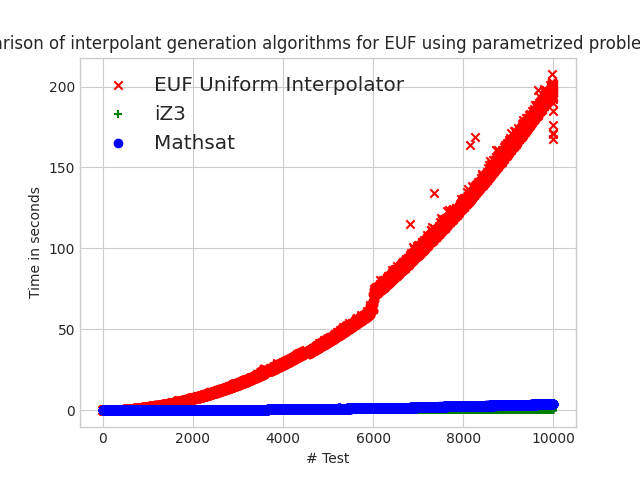
\includegraphics[scale=0.9]{figures/eufi_performance_graph}
  \caption{Performance comparison graph of EUF interpolant generation
  algorithms for paramatrized problem from section \ref{performance_euf}} 
  \label{performance_graph_euf}
\end{figure}

%%% Local Variables:
%%% mode: latex
%%% TeX-master: "main"
%%% End:
